\documentclass{report}
\usepackage[utf8]{inputenc}
\usepackage{underscore}
\usepackage{graphicx}

\title{Map My Garage Sale: User's Guide}
\author{Blake Lowe, Jordan Polaniec}

\begin{document}

\pagenumbering{gobble}
\maketitle
\newpage
\pagenumbering{arabic}

\tableofcontents
\newpage

\chapter{Creating a Map}

Map My Garage Sale will create a blank, new map for you upon starting the application.  

\section{Mapping area configuration}
Your first steps should be selecting a backdrop to display in the background of the mapping area
so you have a proper frame of reference for where things will be shown on your Map.  
This can be done in two places:

\begin{itemize}
\item 
	Clicking the 'Change Backdrop...' button will bring up a dialog to choose an image file to display
behind your mapping area.  This image file must be a PNG file.  Map My Garage Sale will scale the 
image to the size of the mapping area as well.\\

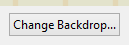
\includegraphics{changebackdropbutton.png}\\

\item
	The other area where the mapping area backdrop can be changed is the File Menu bar.
This is also accessible via keyboard shortcut (SHIFT+S).\\

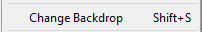
\includegraphics{changebackdropmenu.png}\\

\end{itemize}

Next, if you would like to design your Map without the grid lines present the 'Display Grid' toggle
button can be clicked and the grid lines will no longer be displayed.  Simply clicking the button again will restore
the grid lines.\\

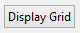
\includegraphics{displaygrid.png}\\

\emph{NOTE} - It's important to remember that these settings are not tied to a specific map and are interchangeable.

\section{Creating your first Stand Template}
Stand Templates are the shapes available to you for placing on the mapping area.  Stands can be used via pre-made
templates included in the application or custom-made by the user.


To create a new Stand Template, click the 'New Stand' button:\\

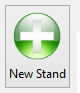
\includegraphics{standtemplatebutton.png}\\


After clicking, the following dialog will be displayed:\\

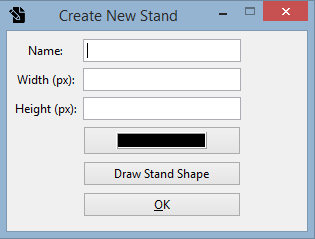
\includegraphics{newstanddialog.png}\\


This dialog gives you all the necessary fields for creating your new custom Stand.  Give it a Name,
dimensions (in pixels) and then click the Color Button (defaults to Black) to select a Color for your Stand.\\


Finally, clicking the 'Draw Stand Shape' button will display a new dialog with a small grid in it.  This is where 
the new shape of your Stand will be created.  Click and hold down the left mouse button to create a 
shape, this is your new stand.  After clicking and dragging the mouse to create said shape, click
 'Done' and your shape will be saved.\\


To wrap up, click 'OK' in the 'Create New Stand' dialog.  Congratulations!  You've created your first 
Stand Template and it is now ready for use in your map!  After you click OK in this dialog, your newly 
minted Stand Template will be displayed in the list of Stand Templates on the right side of the 
main window.  \\

\emph{NOTE} -  Your Stands are specific to the Map you are currently working on and are not shared
across all Maps.\\


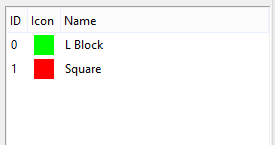
\includegraphics{standtemplateslist.png}\\

\section{Designing your Map}

Now that you have created your stands you are ready to start placing them onto your Map.  
 First select a Stand from the list using the left mouse button and then drag it right into the
 mapping area where you want to place the Stand; a new instance will be created.

Done.  You now have a Stand on your map!  Example:\\

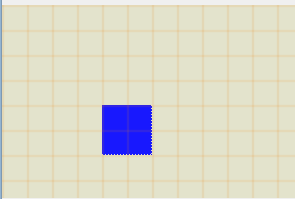
\includegraphics{standingrid.png}\\

Repeat for extent of Map.

\section{Stand adjustments}

 To have a Stand face a different direction or rotate around an object present in 
your backdrop,  click the 'Rotate Stand 90 $^{\circ}$' button:\\

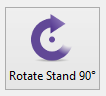
\includegraphics{rotatestandbutton.png}\\

\emph{NOTE} - This will rotate a single Stand and will not affect the Stand Template.

Select a Stand in the mapping area and click this button. The Stand is now rotated 
in the mapping area.

\subsection{Stand Template Management}
Selecting a Stand in the mapping area and select the 'Remove Selected Stand' button to
remove the Stand from the mapping area.\\

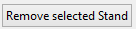
\includegraphics{removestandbutton.png}\\

\emph{NOTE} - This will not delete the Stand Template, only the selected instance of it in the 
mapping area.\\

To delete a Stand Template, select the Stand Template from 
the list on the right then click the 'Delete Stand Template' button:\\

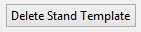
\includegraphics{deletestandtemplatebutton.png}\\

\emph{NOTE} - This is permanent.

Stand Templates can be renamed by double clicking the Name cell of the selected Stand 
Template you would like to modify.  Changing the name and then pressing the 'ENTER' 
key will change the name.\\

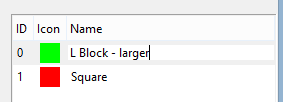
\includegraphics{renamestandtemplate.png}

\subsection{Stand Information}

Information about the currently selected Stand Template can be found in the Metadata bar
located below the list of Stand Templates:\\

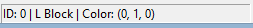
\includegraphics{metadatabar.png}\\

This displays the ID of the Stand Template, the Name and the Color (in RGB format).  

\emph{NOTE} - If the text is longer than what is displayed, hovering the 
mouse over the Metadata bar displays all the information.

\newpage
\chapter{Storage}

\section{Map Management}
Maps are stored in a file with the extension of 'mmgs' (Map My Garage Sale).  Clicking the 
Open File button will bring up a dialog that filters files to show only mmgs files that you have
previously saved:\\

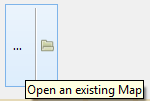
\includegraphics{openfiledialog.png}\\

Opening a file can be done in the File menu bar by clicking the Open File item:\\


\includegraphics{openfilemenuitem.png}\\

\emph{NOTE} - This can be activated via Keyboard shortcut (CTRL+O).\\

To save your work, click the Save button or the Save menu; all saved items will
then be available to open.  :\\

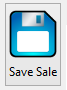
\includegraphics{savebutton.png}\\

Or the Save menu item:
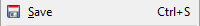
\includegraphics{savemenuitem.png}\\

\emph{NOTE} - This can be activated via Keyboard shortcut (CTRL+S).\\

A brand new Map can be created by clicking the New Map button:\\

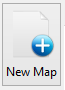
\includegraphics{newmapbutton.png}\\

The New Map menu item can also be used to achieve the same goal:\\

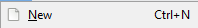
\includegraphics{newmapitem.png}\\

\emph{NOTE} - This can be activated via Keyboard shortcut (CTRL+N).\\

\chapter{Closing}

Congratulations! You now have a solid understanding of how to use Map My Garage Sale.\\

If you have questions for the Developers or need help, feel free to post an issue or comment
on the product github page:\\\\ (https://github.com/thecisguy/map-my-garage-sale).



\end{document}